%%%%%%%%%%%%%%%%%%%%%%%%%%%%%%%%%%%%%%%%%%%%%%%%%%%%%%%%%%%%%%%%%%%%%%%%%%%%%%
%BASE
%%%%%%%%%%%%%%%%%%%%%%%%%%%%%%%%%%%%%%%%%%%%%%%%%%%%%%%%%%%%%%%%%%%%%%%%%%%%%%
\documentclass[11pt,a4paper]{article}%defini caracteristique du document
\usepackage[latin1]{inputenc}
\usepackage{fontenc}
\usepackage[french]{babel} %pour coder en francais%
%%%%%%%%%%%%%%%%%%%%%%%%%%%%%%%%%%%%%%%%%%%%%%%%%%%%%%%%%%%%%%%%%%%%%%%%%%%%%%
%MISE EN PAGE
%%%%%%%%%%%%%%%%%%%%%%%%%%%%%%%%%%%%%%%%%%%%%%%%%%%%%%%%%%%%%%%%%%%%%%%%%%%%%%
\usepackage{lipsum} %pack pour faux text%
\usepackage{ulem}%pour pouvoir souligner
\usepackage{layout}%ajoute les page de description de mise en forme: marges etc
\usepackage[top=2.5cm,bottom=2.5cm,left=2.5cm,right=2.5cm]{geometry}%permet de definir les caracteristique des marges
\usepackage{enumerate}%permet de faire certaine liste comme les articles de lois
\usepackage{paralist}%permet de faire une liste num�rot�e dans un text
\usepackage{graphicx}%permet d'int�grer des figure et graphics
\usepackage{wrapfig}%permet de mettre une photo dans un text
\usepackage{multicol}%permet d'�crire en colonne
\usepackage{subfigure}%permet de mettre deux photos avec une seule l�gende
\usepackage{multirow}%pour faire plusieurs ligne en une dans un tableau
%\usepackage{slashbox}%permet de couper en diagonal la premi�re case en haut �  gauche d'un tableau
\usepackage{array}%permet de rajouter des caract�ristiques pour les colonnes d'un tableau
\usepackage{todonotes}%permet de rajouter des notesii
\usepackage{fancyhdr}%pour entete bas de page et numerotation de page
%%%%%%%%%%%%%%%%%%%%%%%%%%%%%%%%%%%%%%%%%%%%%%%%%%%%%%%%%%%%%%%%%%%%%%%%%%%%%%
%MATHS
%%%%%%%%%%%%%%%%%%%%%%%%%%%%%%%%%%%%%%%%%%%%%%%%%%%%%%%%%%%%%%%%%%%%%%%%%%%%%%
\usepackage{amsmath}%packs pour le mod maths
\usepackage{amssymb}%packs pour le mod maths
\usepackage{amsfonts}%packs pour le mod maths
\DecimalMathComma%pour pr�ciser que d�cimal sont s�par�e par virgule
%%%%%%%%%%%%%%%%%%%%%%%%%%%%%%%%%%%%%%%%%%%%%%%%%%%%%%%%%%%%%%%%%%%%%%%%%%%%%%
%AUTRES
%%%%%%%%%%%%%%%%%%%%%%%%%%%%%%%%%%%%%%%%%%%%%%%%%%%%%%%%%%%%%%%%%%%%%%%%%%%%%%
\usepackage{url}%permet d'insérer des liens
\setlength{\parindent}{0pt}%retire l'indentation
%%%%%%%%%%%%%%%%%%%%%%%%%%%%%%%%%%%%%%%%%%%%%%%%%%%%%%%%%%%%%%%%%%%%%%%%%%%%%%
%DESSIN
%%%%%%%%%%%%%%%%%%%%%%%%%%%%%%%%%%%%%%%%%%%%%%%%%%%%%%%%%%%%%%%%%%%%%%%%%%%%%%
\usepackage{pgfplots}
\usepackage{tikz}
\usepackage[european resistor, european voltage, european current]{circuitikz}
\usetikzlibrary{arrows,shapes,positioning}
\usetikzlibrary{decorations.markings,decorations.pathmorphing,decorations.pathreplacing}
%%%%%%%%%%%%%%%%%%%%%%%%%%%%%%%%%%%%%%%%%%%%%%%%%%%%%%%%%%%%%%%%%%%%%%%%%%%%%%
%ent�te et pied de page
%%%%%%%%%%%%%%%%%%%%%%%%%%%%%%%%%%%%%%%%%%%%%%%%%%%%%%%%%%%%%%%%%%%%%%%%%%%%%%
\pagestyle{fancy} %: Num�rotation des pages.
\lhead{2020-2021} %ent�te et bas de page / haut gauche
\chead{} %haut centre
\rhead{ESAIP} %haut droite
\lfoot{Prise de note: CB} %bas gauche
\cfoot{Data Mining Class} %bas centre
\rfoot{\thepage} %bas droite
%\leftmark: affiche le num et le nom de la section en cours
%\thepage : donne le num de la page
\renewcommand{\headrulewidth}{0.4pt} %: Trace un trait de s�paration de largeur 0,4 point.
%Mettre 0pt pour supprimer le trait.
\renewcommand{\footrulewidth}{0.4pt} %: Trace un trait de s�paration de largeur 0,4 point.
%Mettre 0pt pour supprimer le trait.

\begin{document}
\hrule
\begin{center}
	\begin{Huge}
    Data Mining
	\end{Huge}
\end{center}
\hrule
\tableofcontents

\newpage
\section{Introduction}
\begin{itemize}[\label=\textbullet]
  \item Managing the data (Managing DataBases)
  \item Analysing the data (extract the information)
  \item Reporting the information (Business Intelligence)
\end{itemize}

\subsection*{What is data mining?}
Extract information that was not known before. This extraction is automatic or semi-automatic. The goal is to discover meaningful patterns.\\

It can be divided in 5 parts:
\begin{enumerate}
  \item Input data
  \item Data Preprocessing (feature selection, dimensionality reduction\footnote{Dimension is the number of variables. Visualising more than 3 can be complex, so we need to reduce it to 2 or 3. The most famous algorithm to do so are PCA, T-SNE, LDA}, normalization\footnote{Normalisation is bringing all the value in the same scale 0-1(removing extremums and finding min and max)}, data sub-setting\footnote{Doing the analysing on batches of the database and not all the data at once. Ex: on the first 5 lines, then 5 next, ect \dots})
  \item Data Mining
  \item Post Processing (filtering patterns, visualisation, pattern interpretation)
  \item Information
\end{enumerate}

\subsection*{What is not data mining?}
\begin{itemize}[\label=\textbullet]
  \item Query web search engine
  \item Look up data in database
\end{itemize}

\section{Data Mining Tasks}
\textbf{Prediction Methods}: Use some variables to predict unknown or future values of other variables. (find a function for a correlation between multiples variables and use it to predict the future)\\

\textbf{Description Methods}: Find human interpretable patterns that describe the data\\

But also:
\begin{itemize}
  \item Clustering
  \item Predictive Modeling
  \item Association Rules
  \item Anomaly Detection
\end{itemize}


\newpage
\section{Machine Learning}
\begin{itemize}[\label=\textbullet]
  \item supervised learning \begin{itemize}
                              \item Classification
                              \item Regression
                            \end{itemize}
                        \item Unsupervised learning \begin{itemize} \item Clustering \end{itemize}
  \item Reinforcement Learning
\end{itemize}

\subsection{Predictive Modeling: Classification}
First step is to split the DB in 2: The train dataset and the test dataset (ex: 70\% and 30\%). The 2 sets are randomly selected.\\

!! In Science, splitting randomly is not enough. The model used is the cross-validation (k-fold) and the average of all the set is the result!!  

\begin{figure}[!h]
\begin{center}
  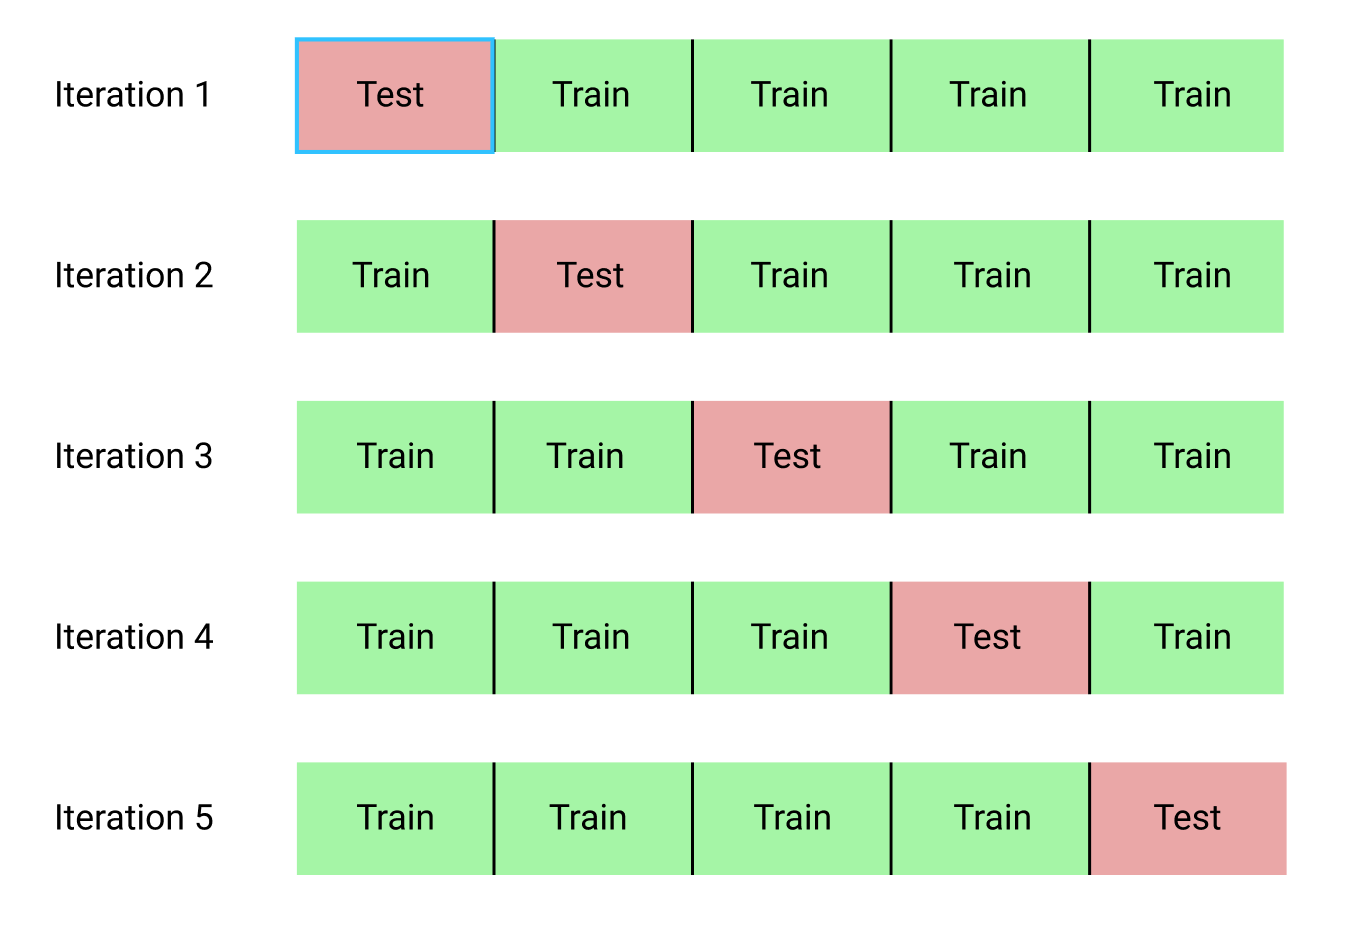
\includegraphics[scale=0.25]{img/k-fold.png}
  \caption{5-fold split}
\end{center}
\end{figure}

Exemple of application: 
\begin{itemize}
\item classifying forest, water bodies, urban area,\dots
\item identify intruder in cyberspaces
\item predicting tumour cells as benign or malignant
\item classifying proteins
\end{itemize}

\subsection{Predictive Modeling: Regression}

Predict a value of a given continuous variable based on other variables assuming a linear or non-linear model of dependency.\\
It's widely studied in statistics.

\subsection{Clustering}
Find group of objects such as distance between object of the same group is small and distance between groups is large.

It can be used to segment the market, group customer by their lifestyle, location, \dots or group product by similarities.


\newpage
\section{AI-900 Azure AI Fundamentals}

\subsection*{What is AI?}
It's a software that can imitate human capabilities and can make decision based on data and experience.

\begin{itemize}
  \item Computer Vision
  \item Neural Language Processing
  \item Conversational AI = BOT
  \item Machine Learning
  \item Anomaly Detection
\end{itemize}

\subsection*{Challenges and risks}
\begin{tabular}{|c|p{9.5cm}|}
\hline
\textbf{Challenge or Risk} & \textbf{Example} \\
\hline
Bias can affect result & discrimination by gender via the data used for the training \\
\hline
Errors may cause harm & autonomous vehicle failure can kill someone\\
\hline
Data could be exposed & sensitive medical data are used to train the data\\
\hline
solution may not work on everyone & a predictive app do not provide audio output for visually deficient people\\
\hline
user must trust a complex system & we don't always understand the AI logic and believing it can be hard\\
\hline
who is liable for AI-driven decision ? & if someone is false accused, who is responsible ?\\
\hline
\end{tabular}

\section{Machine Learning}

For machine learning and computer vision, we have 2 sets of data: train and test. But for deep learning, we need 3 sets of data: train, validation (by back-propagation) and test.

\subsection{Evaluating your model}
To evaluate a model, you can use MAE (Mean absolute error, lower the better) or RMSE (Root mean squared error), RSE (Relative squared error, between 0 and 1, lower is better), $R^{2}$ (closest to 1 the best).

\newpage
\section{Computer Vision}\footnote{see jupyter notebook}

Each image is divided in 3 matrix: RGB.\\
Each matrix is the size of the picture (pixel)and each value is between 0 and 255.

\subsection*{Applications}
\begin{itemize}[\label=\textbullet]
  \item Image classification (label for an image)
  \item Object detection (detect objects on a picture and draw a box arround it)
  \item Semantic segmentation = pixel classification~(object detection pixel sized: the object is highlighted)
  \item image Analysis = image captioning (describe what is in the image)
  \item Face detection \& recognition
  \item Optical character recognition (detect text on picture)
\end{itemize}


\section{NLP (Natural Language Processing)}

\begin{itemize}[\label=\textbullet]
  \item Text Analysis and entity recognition
  \item Sentiment analysis
  \item Speech recognition and synthesis
  \item Machine translation
  \item Semantic language modeling
\end{itemize}

It can be decompose on different field:
\hfill \\

\begin{tabular}{|c|c|}
  \hline
  Text Analytic & Language detection - Key phrase extraction - entity detection - sentiment analysis\\
  \hline
  Speech & Text to speech - speech to text - speech translation\\
  \hline
  Translator text & text translation\\
  \hline
\end{tabular}

\section{Conversation AI (BOT)}

A solution that enable dialogue between AI and human. It's present in mail, web chat, social media, voice.\\

It must respect some principles
\begin{enumerate}
  \item Be transparent about what the BOT can and cannot do
  \item Male it clear that the user is communicating with a BOT
  \item Enable the BOT to give hand to an human
  \item Ensure the BOT respect cultural norms
  \item Ensure the BOT is reliable
  \item Respect user privacy
  \item Handle data securely
  \item Ensure the BOT meet accessibility standards
  \item Assume accountability for the BOT action
\end{enumerate}


\end{document}


